\section{Test af accelerometer} 
\label{sec:test_acc}
I dette projekt anvendes to accelerometre, som er beskrevet i \autoref{sec:acc}. Disse anvendes som sensorer til opsamling af acceleration, der giver et outputsignal svarende til en spænding. For at kunne anvende et accelerometer er det vigtigt at kende forskellige tolerancer i forhold til deres datablade, hvorfor et forsøg udføres for at kunne tage højde for disse parametre.

\subsection{Formål}\label{sec:acc_formaal}
Denne test har til formål at identificere en given spændingen for forskellige vinkler. Derudover identificeres %støjsignaler i outputsignalet samt 
offsettet og sensitiviteten for at teste accelerometrenes tolerancer.

\begin{enumerate}
%\item Identificering af støj i outputsignaler for accelerometrene
\item Test af linearitet
\item Identificering af offsettet og sensitiviteten for accelerometrene
\item Identificering af spænding ved forskellige vinkler
\end{enumerate}

\subsection{Materialer}
\begin{itemize}
\item Accelerometre ADXL$335$
\item Tape
\item Vaterpas
\item Breadboard
\item LEGO-model, fremgår af \autoref{fig:vinkeltest}
\item Computer med Scopelogger og MATLAB
\item NI USB-6009
\end{itemize}

\subsection{Metode}
Der opstilles en metode til hvert formål i \autoref{sec:acc_formaal}. Formål 1 opfyldes ved deltest 1, og formål 2 og 3 opfyldes ved deltest 2. 
\begin{enumerate}
%\item Der foretages målinger i accelerometerets tre akser og i de seks positioner som accelerometeret, hvorved støj som accelerometeret påvirkes med kan identificeres
\item Der foretages målinger i accelerometerets tre akser i 11 positioner, hvorved der kan testes for linearitet
\item Der foretages målinger i accelerometerets tre akser i de seks positioner, hvorefter offset og sensitiviteten kan beregnes ud fra målingerne. Offsettet beregnes ud fra accelerometerets 0 g-påvirkning, der måles vinkelret på planet, hvilket svarer til at accelerometeret ikke udsættes for tyngdekraften. Sensitiviteten måles ud fra en 1 g-påvirkning
\item Ud fra målingerne ved 0 og 1 g-påvirkning kan spændingen ved $1^{\circ}$ og $90^{\circ}$ kan beregnes ved \autoref{equ:vinkler}
\end{enumerate}

\subsection{Forsøgsopstilling}
Forsøgsopstillingen udføres på samme måde for begge accelerometre.

\subsubsection{Forsøgsopstilling af deltest 1}
\begin{itemize}
\item Accelerometeret påsættes LEGO-modellen på \autoref{fig:vinkeltest}
\begin{itemize}
\item Accelerometeret indstilles efter fremgangsmåden for hver øvelse som er illustreret i \autoref{sec:vinkel_fremgangsmaade}
\end{itemize}
\item Accelerometeret tilkobles NI USB-6009
\item NI USB-6009 tilkobles en computer
\end{itemize}

\subsubsection{Forsøgsopstilling af deltest 2}
\begin{itemize}
\item Accelerometeret påsættes breadboardet og fastsættes med tape
\item Accelerometeret indstilles, så det er i vater med et vaterpas
\begin{itemize}
\item Accelerometeret placeres efter fremgangsmåden for hver øvelse, hvilket er illustreret i \autoref{sec:acc_fremgangsmaade}
\end{itemize}
\item Accelerometeret tilkobles NI USB-6009
\item NI USB-6009 tilkobles en computer
\end{itemize}

\subsection{Fremgangsmåde}  

\subsubsection{Fremgangsmåde for deltest 1} \label{sec:vinkel_fremgangsmaade}
Hver vinkel måles og samples for hvert accelerometer i hver akse i 10 sekunder ved $100~Hz$, hvilket er det dobbelte af båndbredden for accelerometrene \citep{analogdevices2010}. Målingerne er udført for begge accelerometre i henholdsvis x-, y- og z-aksen, og vinklen ændres ved at justere LEGO-modellen på \autoref{fig:vinkeltest}, så følgende vinkler fremgår af modellen:
\begin{itemize}
\item $0^{\circ}$ til $180^{\circ}$ med $20^{\circ}$'s intervaller
\item $90^{\circ}$  
\end{itemize}


\begin{figure}[H]
\centering
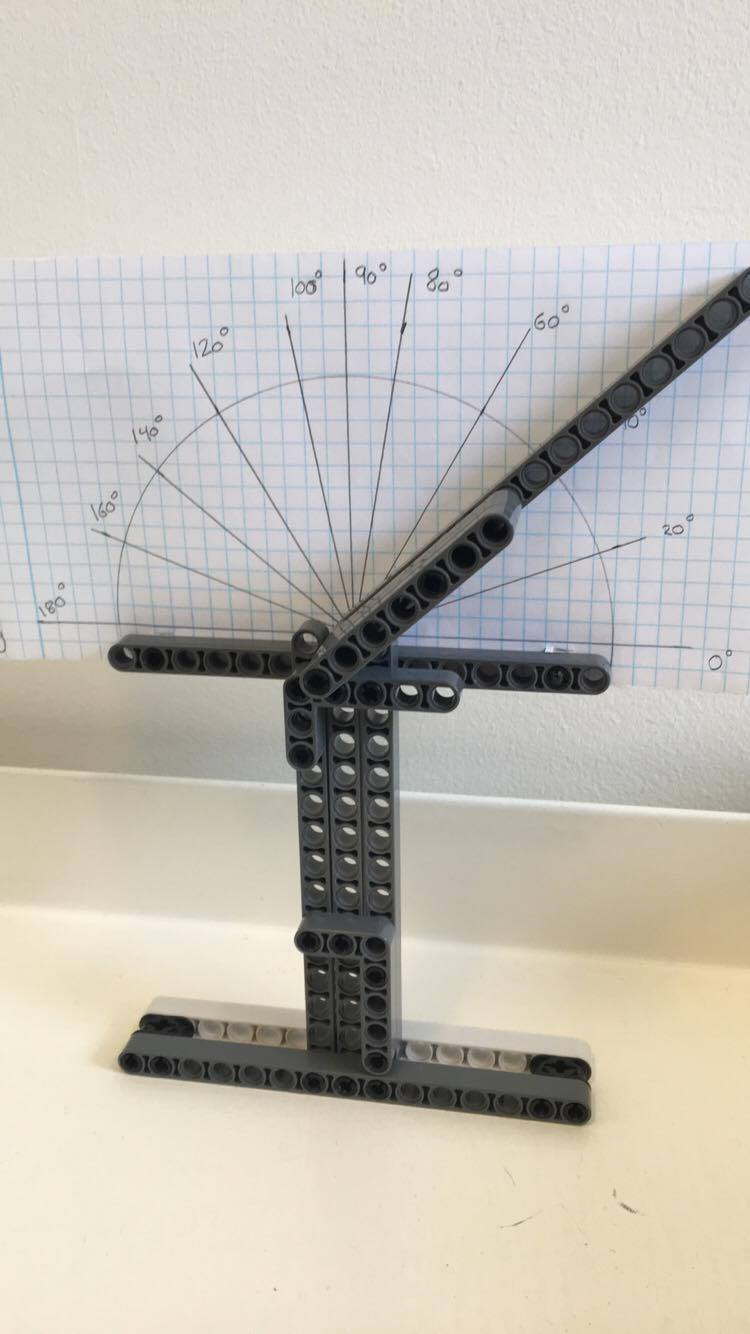
\includegraphics[width=0.3\textwidth]{figures/vinkeltest}
\caption{Vinkeltester, som anvendes under forsøget til at holde accelerometeret i bestemte vinkler.}
\label{fig:vinkeltest}
\end{figure}

\subsubsection{Fremgangsmåde for deltest 2}\label{sec:acc_fremgangsmaade}
Der foretages målinger i seks forskellige positioner. Hver position måles tre gange og samles i 10 sekunder ved $100~Hz$. De forskellige positioner er illustreret på \autoref{fig:acc_paavirkning}, og er som følger: 
\begin{itemize}
\item Accelerometeret stilles, så det er lodret opad
\item Accelerometeret stilles, så det er lodret nedad
\item Accelerometeret stilles, så det er vandret mod højre
\item Accelerometeret stilles, så det er vandret mod venstre
\item Accelerometeret ligges plan på bordet med toppen opad
\item Accelerometeret ligges plan på bordet med toppen nedad
\end{itemize}

\begin{figure}[H]
\centering
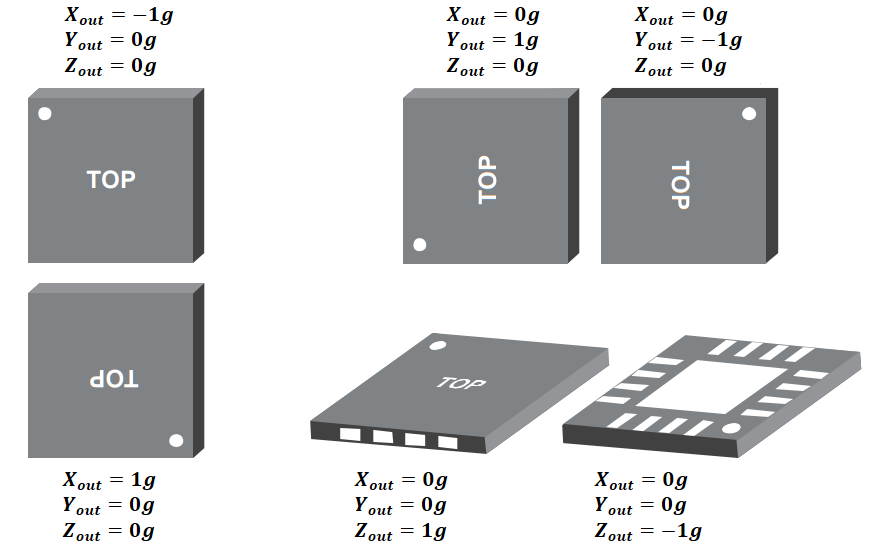
\includegraphics[width=0.5\textwidth]{figures/acc_paavirkning}
\caption{Påvirkning af accelerometeret i forskellige positioner. Til venstre måles accelerometeret i lodret plan, til højre øverst vandret og til højre nederst i plan \citep{analogdevices2010}.}
\label{fig:acc_paavirkning}
\end{figure}

\subsection{Resultater} 

\subsubsection{Resultater for deltest 1}
For deltest 1 udføres en lineær regression, hvor data fra målingerne af begge accelerometres output ved hver målt vinkel plottes som en funktion af vinklerne. Derefter udføres den lineære regression, og $R^2$-værdien findes, så det kan bestemmes, om punkterne er lineære. Plots, regressioner og $R^2$-værdier kan ses på \autoref{fig:acc_lineaerregression}.

\begin{figure}[H]
\centering
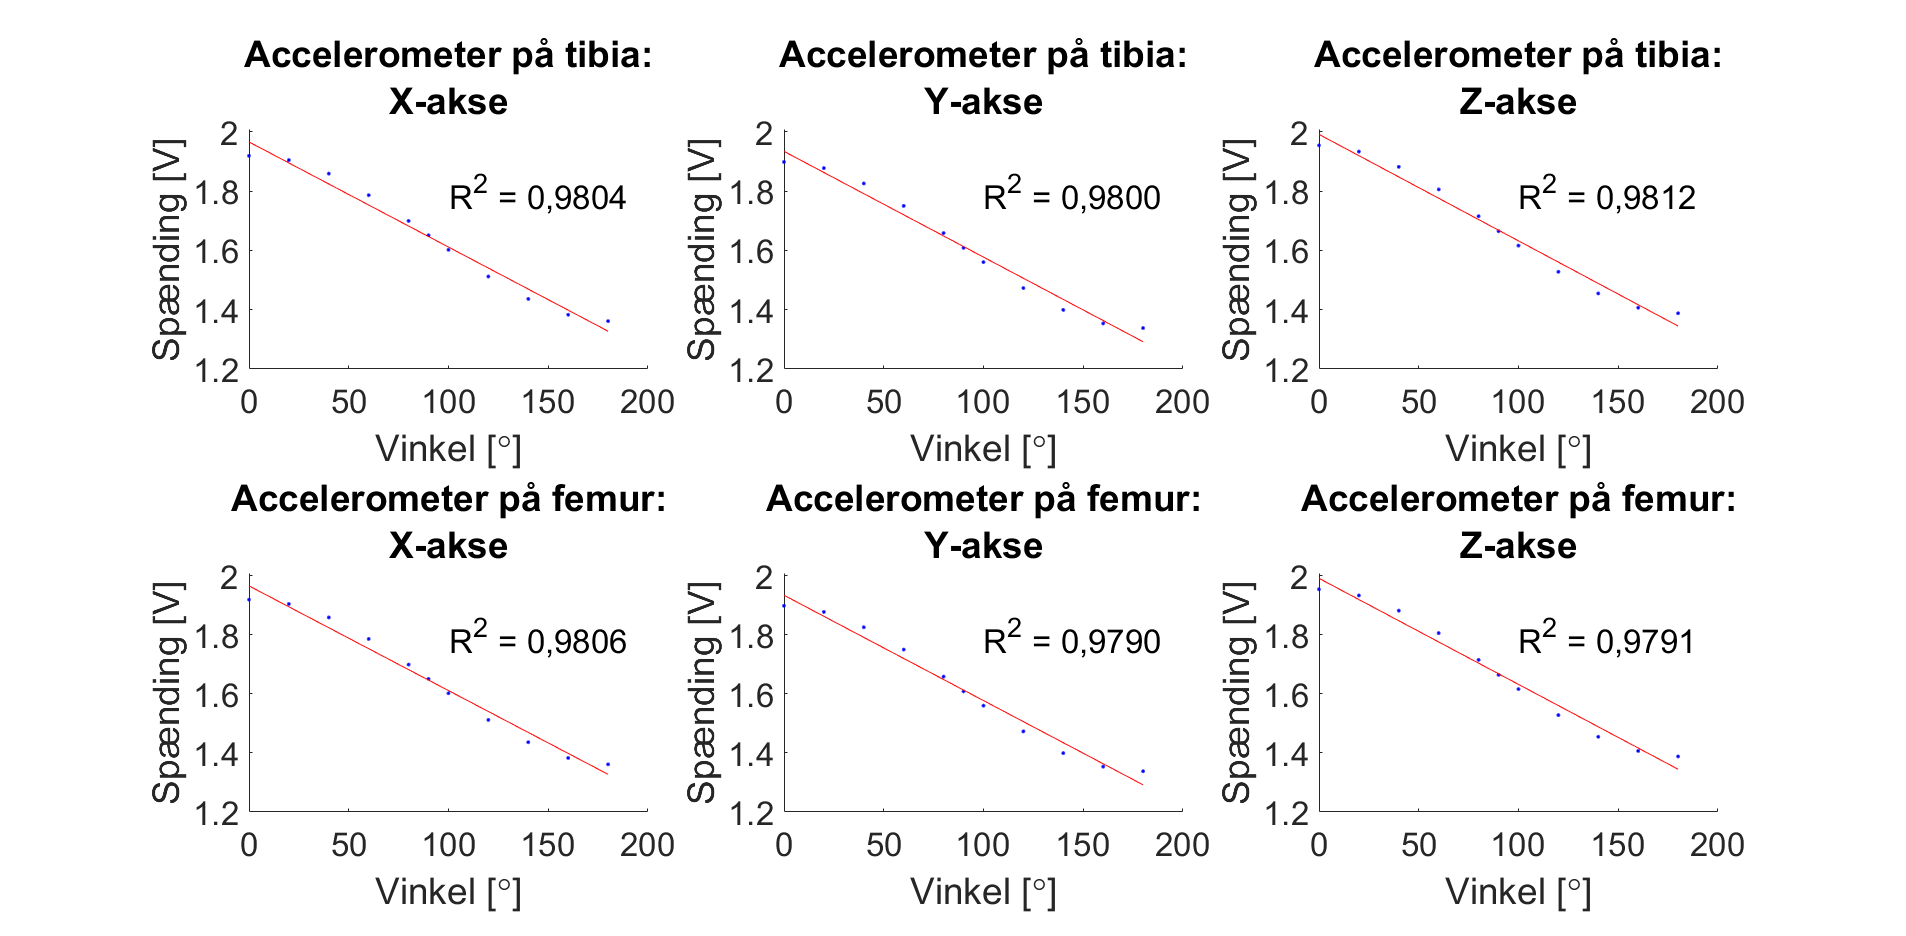
\includegraphics[width=0.9\textwidth]{figures/lineaerregression}
\caption{Lineær regression for hver akse på hvert accelerometer. Målingerne er plottet med blå prikker, og den lineære regression er illustreret med rød. $R^2$-værdien er noteret for hvert plot.}
\label{fig:acc_lineaerregression}
\end{figure}

Ud fra \autoref{fig:acc_lineaerregression} kan det ses, at $R^2$-værdierne er mellem 0,9790 og 0,9812. Graferne ville have en perfekt lineær sammenhæng, hvis $R^2=1$. Det kan derfor siges, at der her ses en lineær tendens ud fra disse målinger, selvom punkterne på alle seks grafer viser en s-formet bølge omkring regressionslinjen, hvilket giver afvigelserne fra den perfekte lineære sammenhæng.

\subsubsection{Resultater for deltest 2}
De viste resultater heri er for det ene accelerometer\fxnote{resultaterne er fra det røde accelerometer}, da sensitiviten og offsettet ændrer sig hver gang, der udføres et forsøg. Det vil derfor ikke være muligt at fastsætte konstante værdier for sensitivitet og offset, hvorfor det centrale at udlede er metoden til at beregne værdierne, da udregningerne skal foretages ved hvert forsøg.

Ud fra de tre målinger foretaget i de seks forskellige positioner beregnes den gennemsnitlige værdi af målingerne på de forskellige akser, herefter plottes disse i en graf. På denne måde bliver det muligt at se, hvilken akse der påvirkes mest under øvelsen. Målingerne fremgår af \autoref{fig:acc_paavirkning2}. 

\begin{figure}[H]
\centering
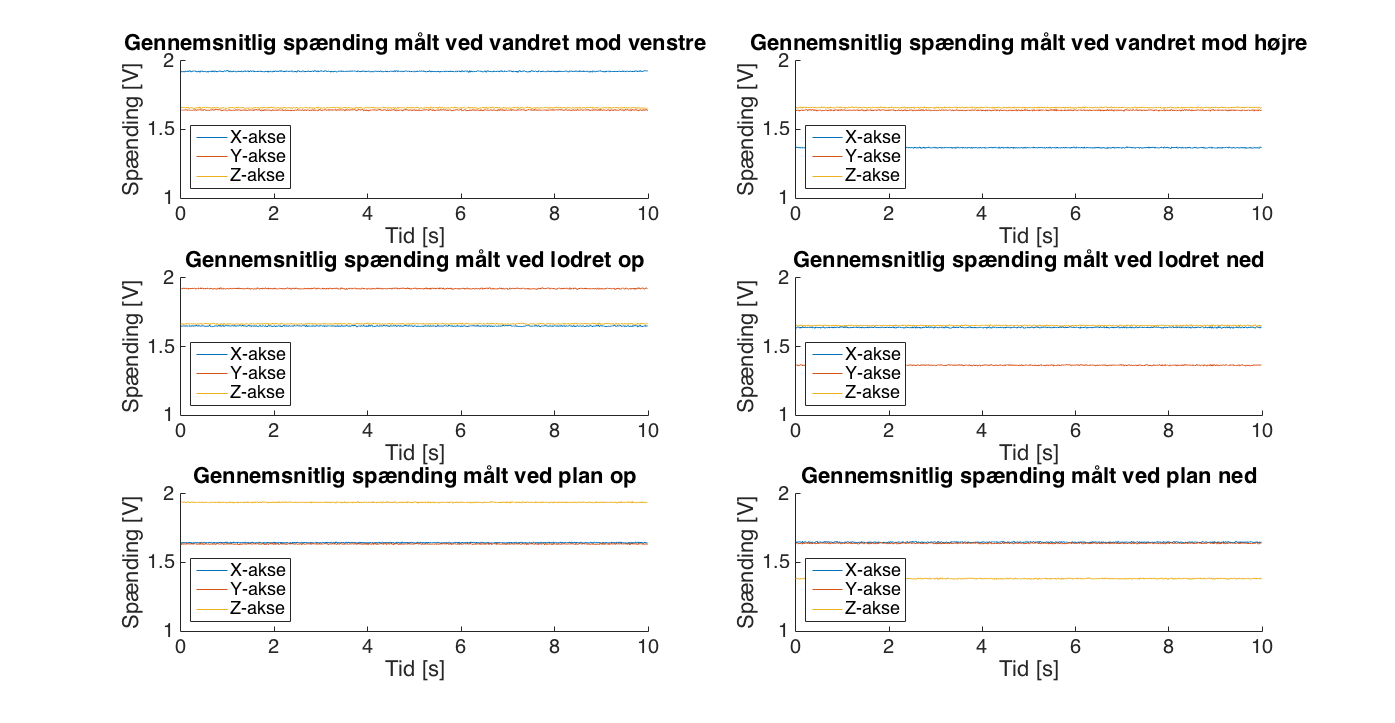
\includegraphics[width=0.8\textwidth]{figures/paavirkning}
\caption{Påvirkningen af accelerometrets tre akser ved de seks forskellige positioner.}
\label{fig:acc_paavirkning2}
\end{figure}

Offset beregnes ud fra de målinger, hvor accelerometeret påvirkes med 0 g. Den akse hvor accelerometeret påvirkes med 0 g i alle seks forskellige positioner fremgår af \autoref{fig:acc_paavirkning}. Resultaterne fra målingerne fremgår af \autoref{tab:acc_offset}. 

\begin{table}[H]
	\centering
	\begin{tabular}{|l|l|l|}
	\textbf{Målt retning} & \textbf{Målt akse} & \textbf{Offset} \\ \hline
    \textbf{Lodret op} 		& X 		& $1,6793~V$ 	\\ \hline
    \textbf{Lodret op} 		& Z 		& $1,6857~V$ 	 \\ \hline
    \textbf{Lodret ned}		& X 		& $1,6750~V$ 	\\ \hline
    \textbf{Lodret ned}		& Z 		& $1,6806~V$  	\\ \hline
    \textbf{Vandret højre} 	& Y 		& $1,6760~V$    \\ \hline     
    \textbf{Vandret højre} 	& Z 		& $1,6828~V$ 	\\ \hline
    \textbf{Vandret venstre}	& Y 		& $1,6755~V$ 	\\ \hline
    \textbf{Vandret venstre}	& Z 		& $1,6836~V$		\\ \hline
    \textbf{Plan op} 		& X 		& $1,6773~V$		\\ \hline		
    \textbf{Plan op} 		& Y 		& $1,6734~V$    \\ \hline
    \textbf{Plan ned} 		& X 		& $1,6787~V$		\\ \hline
    \textbf{Plan ned} 		& Y 		& $1,6755~V$		\\ \hline
	\end{tabular}
	\caption{Offsettet beregnet for de forskellige akser, hvor accelerometeret udsættes for en 0 g-påvirkning.}
	\label{tab:acc_offset}
\end{table}

Sensitiviten beregnes ud fra forskellen mellem 0 og 1 g-påvirkningen af accelerometeret. Der hvor accelerometeret er påvirket med 1 g er illustreret på \autoref{fig:acc_paavirkning}. Målingerne fremgår af \autoref{tab:acc_sensitivitet}. 

\begin{table}[H]
	\centering
	\begin{tabular}{|l|l|l|}
	\textbf{Målt retning} & \textbf{Målt akse} & \textbf{Sensitivitet} \\ \hline
    \textbf{Lodret op} 		& Y		& $0,1092~V/g$ 	\\ \hline
    \textbf{Lodret ned}		& Y 		& $-0,1164~V/g$ 	\\ \hline
    \textbf{Vandret højre} 	& X 		& $0,1130~V/g$     \\ \hline     
    \textbf{Vandret venstre}	& X 		& $-0,1167~V/g$ 	\\ \hline
    \textbf{Plan op} 		& Z 		& $0,1232~V/gV$    	\\ \hline		
    \textbf{Plan ned} 		& Z 		& $-0,1079~V/g$		\\ \hline
	\end{tabular}
	\caption{Sensitiviteten beregnet for de forskellige akser hvor accelerometeret udsættes for en 1 g-påvirkning.}
	\label{tab:acc_sensitivitet}
\end{table}

Ud fra senstitivten beregnes spændingen ved $1^{\circ}$ og $90^{\circ}$ i negativ og positiv retning\fxnote{Er der nødvendig med 1 grad?}. Spændingen svarende til $0^{\circ}$ svarer til den målte offsetværdi som fremgår af \autoref{tab:acc_offset}. Udregningerne af spænding ved de valgte grader fremgår af \autoref{tab:acc_grader} og er beregnet ud fra ligning \autoref{equ:vinkler}.

 \begin{table}[H]
	\centering
	\begin{tabular}{|l|l|l|l|}
	\textbf{Målt retning} & \textbf{Målt akse} & \textbf{Spændingen ved $1^{\circ}$} & \textbf{Spændingen ved $90^{\circ}$} \\ \hline
    \textbf{Positiv} 	& Y		& $1,7985~V$   	&	$12,7589~V$\\ \hline
    \textbf{Negativ}		& Y		& $1,5692~V$  	&	$-8,0339~V$\\ \hline
    \textbf{Positiv} 	& X 		& $1,7917~V$   	& 	$11,5105~V$ \\ \hline     
    \textbf{Negativ}		& X 		& $1,5614~V$		&	$-8,7982~V$\\ \hline
    \textbf{Positiv} 	& Z 		& $1,7924~V$   	& 	$11,8494~V$	\\ \hline		
    \textbf{Negativ} 	& Z 		& $1,5629~V$		&	$-8,8190~V$ \\ \hline
	\end{tabular}
	\caption{Beregnet spænding ved henholdsvis $1^{\circ}$ og $90^{\circ}$ i positiv og negativ retning.}
	\label{tab:acc_grader}
\end{table}





